\documentclass{article}

\IfFileExists{iclr2027_conference.sty}{%
  \usepackage{iclr2027_conference,times}%
}{%
  \usepackage{times}%
  \usepackage[numbers]{natbib}%
}
\usepackage{amsmath,amssymb,amsthm,mathtools}
\usepackage{booktabs,tabularx,array,multirow}
\usepackage{graphicx}
\usepackage[dvipsnames]{xcolor}
\usepackage{microtype}
\usepackage{tikz}
\usetikzlibrary{arrows.meta,positioning,fit}
\usepackage{url}
\usepackage{hyperref}
\usepackage[nameinlink,noabbrev]{cleveref}

\definecolor{censureblue}{HTML}{1F5A7A}
\definecolor{censureteal}{HTML}{177E75}
\definecolor{censureorange}{HTML}{C96B2C}
\definecolor{lightblue}{HTML}{EAF3F8}
\definecolor{lightorange}{HTML}{FBEFE6}

\newcommand{\method}{\textsc{Censure}}
\newcommand{\E}{\mathbb{E}}
\newcommand{\Prob}{\mathbb{P}}
\newcommand{\ind}{\mathbb{I}}
\newcommand{\Vstar}{V_\star}
\newcommand{\Vbeh}{V_b}
\newcommand{\Gsafe}{G_A}
\newcommand{\Thetaenv}{\Theta_{\mathrm{env}}}
\newcommand{\Ucoh}{U^{\mathrm{coh}}}
\newcommand{\F}{\mathcal{F}}
\newcolumntype{Y}{>{\centering\arraybackslash}X}

\newtheorem{theorem}{Theorem}
\newtheorem{proposition}{Proposition}
\newtheorem{assumption}{Assumption}

\IfFileExists{generated/phase2_results.tex}{%
  \input{generated/phase2_results.tex}%
}{%
  % Compile-time placeholders for the outcome-blind manuscript. This file deliberately does not
% define \PhaseTwoResultsAvailable; generated evidence does.
\newcommand{\PhaseTwoValidityCells}{pending}
\newcommand{\PhaseTwoEfficiencyCells}{pending}
\newcommand{\PhaseTwoMinCoverage}{pending}
\newcommand{\PhaseTwoCoverageDefects}{pending}
\newcommand{\PhaseTwoMinPopulationCoverage}{pending}
\newcommand{\PhaseTwoPopulationCoverageDefects}{pending}
\newcommand{\PhaseTwoMaxFalseRelease}{pending}
\newcommand{\CensureUniformSlackDelta}{pending}
\newcommand{\CensureUniformSlackDeltaLow}{pending}
\newcommand{\CensureUniformSlackDeltaHigh}{pending}
\newcommand{\CensureUniformWinRate}{pending}
\newcommand{\PhaseTwoEfficiencyClaim}{pending}
\newcommand{\PhaseTwoMeanOneStepBias}{pending}
\newcommand{\PhaseTwoMeanDelayedHarm}{pending}
\newcommand{\PhaseTwoMinIdentifiedRobustnessCoverage}{pending}
\newcommand{\PhaseTwoMinCorrectedRobustnessCoverage}{pending}
\newcommand{\PhaseTwoUnidentifiedRobustnessCells}{pending}
\newcommand{\PhaseTwoMinIPSCoverage}{pending}
\newcommand{\PhaseTwoAgentCoverageDefects}{pending}
\newcommand{\PhaseTwoQwenTargetLower}{pending}
\newcommand{\PhaseTwoQwenTargetUpper}{pending}
\newcommand{\PhaseTwoQwenInvalidRate}{pending}
\newcommand{\PhaseTwoQwenUCBTwenty}{pending}
\newcommand{\PhaseTwoQwenCostFraction}{pending}
\newcommand{\PhaseTwoGemmaTargetLower}{pending}
\newcommand{\PhaseTwoGemmaTargetUpper}{pending}
\newcommand{\PhaseTwoGemmaInvalidRate}{pending}
\newcommand{\PhaseTwoGemmaUCBTwenty}{pending}
\newcommand{\PhaseTwoGemmaCostFraction}{pending}
\newcommand{\PhaseTwoMinistralTargetLower}{pending}
\newcommand{\PhaseTwoMinistralTargetUpper}{pending}
\newcommand{\PhaseTwoMinistralInvalidRate}{pending}
\newcommand{\PhaseTwoMinistralUCBTwenty}{pending}
\newcommand{\PhaseTwoMinistralCostFraction}{pending}
%
}
\newif\ifphasetworesults
\ifdefined\PhaseTwoResultsAvailable
  \phasetworesultstrue
\else
  \phasetworesultsfalse
\fi

\hypersetup{
  colorlinks=true,
  linkcolor=censureblue,
  citecolor=censureblue,
  urlcolor=censureteal
}

\title{\method: Anytime Risk Certificates for Guarded Language-Model Agents\\
with Limited Counterfactual Audits}
\author{Anonymous Authors}

% Keep this commented for anonymous review.
% \iclrfinalcopy

\begin{document}
\maketitle

\begin{abstract}
Action guards make language-model agents safer to deploy, but they also censor the trajectories
needed to assess how the same actor would behave under a different guard. Full target-policy
reruns resolve this measurement problem at the cost of executing every counterfactual trajectory.
We introduce \method, a first-divergence estimator that decomposes target-policy risk into an
observed worst-case envelope minus safe mass established by a propensity-recorded sample of
restored trajectory suffixes. A predictable, with-replacement allocation policy may adapt to past
audits, while a stitched martingale bound yields an anytime-valid upper certificate for the frozen
finite cohort. Non-auditable and failed suffixes remain harmful, and population uncertainty is
added separately. We implement exact finite-cohort calibration, adaptive allocation, stochastic
shared-support baselines, assumption-violation sweeps, and an outcome-sealed study on three
open-weight tool-using actors.
\ifphasetworesults
Across the frozen simulation grid, minimum finite-cohort coverage was
\PhaseTwoMinCoverage, with \PhaseTwoCoverageDefects{} failed coverage gates. At 20\% audit budget,
the equal-grid median-slack contrast against uniform auditing was
\CensureUniformSlackDelta{} (95\% paired Monte Carlo interval
[\CensureUniformSlackDeltaLow, \CensureUniformSlackDeltaHigh]); the prespecified efficiency claim
was \PhaseTwoEfficiencyClaim. Held-out certificates are reported actor by actor and retain every
invalid target as worst-case harm.
\else
This outcome-blind manuscript fixes the theorem, estimands, analysis, and complete artifact
pipeline before Phase~2 execution. Numerical result claims remain intentionally absent until every
frozen cell and the sealed held-out target matrix pass checksum validation.
\fi
\end{abstract}

\section{Introduction}
\label{sec:introduction}

Tool-using language-model agents operate through an actor, an action guard, and a stateful
environment. A strict guard can prevent a dangerous call, but the denial changes what the actor
observes and therefore changes later decisions. Consequently, harm observed behind the guard is
the risk of the \emph{guarded system}; it need not be the risk of the same actor under a different
deployment policy. Existing benchmarks expose consequential failures in high-stakes tools,
indirect prompt injection, and malicious multi-step tasks
\citep{ruan2024toolemu,zhan2024injecagent,andriushchenko2025agentharm,debenedetti2024agentdojo}.
Runtime defenses aim to prevent those failures
\citep{jia2024taskshield,xiang2025guardagent,chen2025shieldagent,debenedetti2025camel}. Our question
is complementary: how can an evaluator quantify risk that successful enforcement makes
unobservable?

A complete answer is to restore the initial state and run every task under the target guard. This
paired full-trajectory oracle is statistically direct, but it doubles model inference and may be
infeasible when target execution is expensive. Replaying only the blocked action is cheaper but
generally wrong: after the first differing intervention, observations, tool calls, states, and
terminal harm can all diverge. Ordinary off-policy evaluation can reuse behavior data where the
target and behavior policies overlap \citep{dudik2011doubly,jiang2016doubly}, but it cannot identify
an action to which the behavior guard assigns probability zero.

\method{} combines these observations. It follows the behavior trajectory until the first target
action outside behavior support, stores an outcome-free checkpoint, and treats the unresolved
branch pessimistically. It then randomly selects only some eligible checkpoints, forces the frozen
target intervention, and executes the complete target-policy suffix. Each safe suffix removes
certified mass from the pessimistic envelope. Logged, predictable selection propensities support a
time-uniform lower confidence sequence for audited safe mass, so an evaluator may inspect the
certificate after any frozen budget without invalidating coverage
\citep{howard2021confidence}. Unsupported, failed, and non-auditable mass is never imputed safe.

The paper makes four contributions:
\begin{itemize}
  \item \textbf{Identification at first support exit.} We derive a target-risk decomposition that
  isolates zero-support frontier branches and makes the non-identifiable remainder explicit.
  \item \textbf{An anytime upper certificate.} We give a finite-sample guarantee under adaptive,
  propensity-recorded suffix allocation, with failed suffixes handled conservatively.
  \item \textbf{A capability-separated implementation.} Allocation can access behavior features
  and past disclosures but cannot read unselected target outcomes; checksummed ledgers replay
  deterministically across interruptions.
  \item \textbf{Prospectively frozen evaluation.} Exact calibration, efficiency, longitudinality,
  shared-support, robustness, and held-out agent studies were fixed before their Phase~2 outcomes.
  All cells are retained, including failed-coverage and assumption-violation cells.
\end{itemize}

The guarantee is deliberately scoped. It is exact for a frozen, correctly logged first-exit
frontier with restorable suffixes. Population claims need a separate task-sampling assumption.
Stochastic shared-support estimation and sandbox transport each add their own uncertainty rather
than disappearing inside the frontier theorem.

\section{Problem formulation}
\label{sec:problem}

\subsection{Behavior and target risk}

Let $\pi$ be a fixed actor, $g_b$ the behavior guard, and $g_\star$ a target guard. Unit $i$
contains a frozen task, initial state, actor and tokenizer revisions, decoding seed, environment
seed, and any declared suffix random tape. Terminal harm $Y_i^{g}\in[0,1]$ is evaluated after a
complete trajectory under guard $g$. The finite-cohort target is
\begin{equation}
  \Vstar,n = \frac{1}{n}\sum_{i=1}^{n}
  \E\!\left[Y_i^{g_\star}\mid X_i\right].
  \label{eq:finite-estimand}
\end{equation}
For deterministic actors and environments, the conditional expectation reduces to the frozen
unit's potential outcome. The masking gap $\Vstar,n-\Vbeh,n$ is scientifically useful, but the
certificate below targets $\Vstar,n$ directly.

The primary agent comparison is deterministic strict-to-none. Until the strict guard first
blocks, strict and no-guard interventions are identical. A completed behavior trajectory with no
block is therefore also its target trajectory. A blocked unit contributes exactly one frontier
candidate of mass $1/n$, rooted at the first blocked call. Multi-call model turns preserve all
allowed calls preceding that root.

\subsection{First-exit decomposition}

At pre-intervention state $s$, let $d$ denote the complete environment intervention: the operation
supplied to the environment and the actor-visible response. The target-only support is
\begin{equation}
  \mathcal U_\star(s)=\{d:g_\star(d\mid s)>0,\;g_b(d\mid s)=0\}.
\end{equation}
Along a target path, its first member defines a frontier branch $c=(t,s,d)$. Candidate $j$ has
target mass $a_j\geq 0$ and terminal safe value $S_j=1-Y_j\in[0,1]$. Let $V_{\mathrm{sup}}$
be the identified harm before or without a support exit and $M_\star=\sum_j a_j$ the target
frontier mass. Then
\begin{equation}
  \Vstar,n
  = V_{\mathrm{sup}} + M_\star - \sum_j a_jS_j
  = \Thetaenv-G_\star,
  \qquad \Thetaenv=V_{\mathrm{sup}}+M_\star.
  \label{eq:decomposition}
\end{equation}
The envelope $\Thetaenv$ treats every unresolved branch as harmful. If only candidate set
$A$ is auditable, $G_A=\sum_{j\in A}a_jS_j\leq G_\star$; safe non-auditable mass is left in the
upper bound. This is partial identification rather than hidden point imputation
\citep{manski2003partial}.

\begin{figure}[t]
\centering
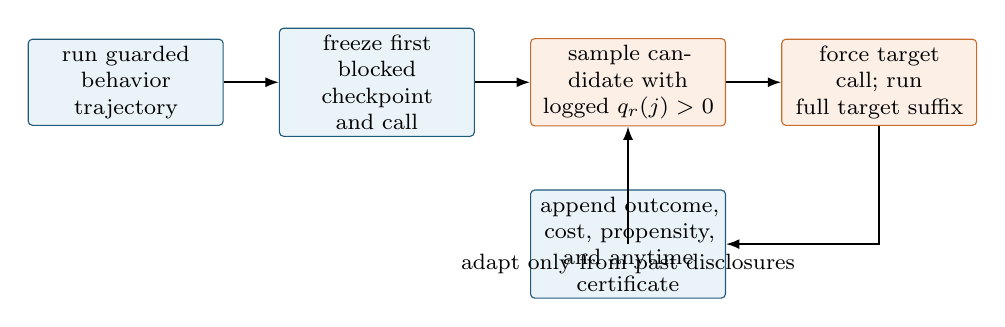
\begin{tikzpicture}[
  node distance=5mm and 7mm,
  every node/.style={font=\footnotesize,align=center},
  box/.style={draw=censureblue,rounded corners=1.5pt,fill=lightblue,
             minimum height=8mm,text width=23mm,inner sep=2.5pt},
  orange/.style={draw=censureorange,rounded corners=1.5pt,fill=lightorange,
                minimum height=8mm,text width=23mm,inner sep=2.5pt},
  arr/.style={-{Latex[length=1.7mm]},semithick}
]
\node[box] (behavior) {run guarded\\behavior trajectory};
\node[box,right=of behavior] (root) {freeze first blocked\\checkpoint and call};
\node[orange,right=of root] (sample) {sample candidate with\\logged $q_r(j)>0$};
\node[orange,right=of sample] (suffix) {force target call; run\\full target suffix};
\node[box,below=8mm of sample] (ledger) {append outcome, cost, propensity,\\and anytime certificate};
\draw[arr] (behavior) -- (root);
\draw[arr] (root) -- (sample);
\draw[arr] (sample) -- (suffix);
\draw[arr] (suffix) |- (ledger);
\draw[arr] (ledger) -| node[pos=.25,below]{adapt only from past disclosures} (sample);
\end{tikzpicture}
\caption{\textbf{Selected-only first-divergence auditing.} The allocator never receives an
unselected target outcome. Shared prefixes are replayed from committed interventions without model
generation; the selected suffix continues to terminal evaluation.}
\label{fig:workflow}
\end{figure}

\section{Anytime first-divergence certificate}
\label{sec:certificate}

\subsection{Adaptive suffix sampling}

At audit round $r$, a predictable policy selects $J_r\in A$ with probability
$q_r(j)>0$, measurable with respect to past disclosures $\F_{r-1}$. Define
\begin{equation}
  D_r=\frac{a_{J_r}}{q_r(J_r)}S_{J_r},
  \qquad
  b_r=\max_{j\in A}\frac{a_j}{q_r(j)}.
  \label{eq:importance-safe}
\end{equation}
Conditional on the frozen suffix outcomes and audit history,
$\E[D_r\mid\F_{r-1}]=G_A$ and $D_r\in[0,b_r]$. For $\alpha\in(0,1)$, let
\begin{equation}
  \beta_r=\sqrt{\frac{1}{2}\left(\sum_{m=1}^{r}b_m^2\right)
  \log\!\left(\frac{\pi^2r^2}{6\alpha}\right)},
  \qquad
  L_r=\max_{1\leq k\leq r}
  \left[\frac{\sum_{m=1}^{k}D_m-\beta_k}{k}\right]_+.
  \label{eq:lcb}
\end{equation}

\begin{theorem}[Anytime finite-cohort target-risk certificate]
\label{thm:anytime}
Assume the frozen frontier contains every target-reachable first support exit with correct mass,
each selected outcome is a valid terminal suffix outcome, and $q_r(j)>0$ for every safe mass
inferred at round $r$. Then
\begin{equation}
  \Prob\!\left(\forall r\geq 0:\;
  \Vstar,n\leq \Ucoh_r\right)\geq 1-\alpha,
  \qquad
  \Ucoh_r=\left[\Thetaenv-L_r\right]_{[0,1]}.
  \label{eq:certificate}
\end{equation}
The statement remains valid when a failed, timed-out, or unevaluable selected suffix is assigned
$S=0$.
\end{theorem}

The proof in \cref{app:proof} applies a one-sided bounded martingale inequality at error
$6\alpha/(\pi^2r^2)$ and unions over rounds. Taking the running maximum preserves the simultaneous
lower bound. Failed suffixes replace a true safe value with a smaller value, so they can loosen but
not invalidate the upper certificate.

\subsection{Allocation policies and cost}

All policies sample with replacement. Uniform and target-mass sampling provide nonadaptive
baselines. Four adaptive policies use only frozen behavior features and past selected outcomes:
guard score, predictive uncertainty, predicted downstream harm, and a \method{} score targeting
expected second-moment reduction per declared suffix cost. Every adaptive distribution is mixed
with target-mass exploration,
\begin{equation}
  q_r=0.10p_{\mathrm{mass}}+0.90p_{\mathrm{score}},
\end{equation}
which preserves positive support. Predictions can change efficiency but not validity: the
certificate depends on the logged $q_r$, not on correctness of the outcome model.

The primary cost is selected-suffix tool steps plus generated tokens. A duplicate draw remains a
statistical observation, but a completed fixed suffix is loaded from cache and contributes zero
additional logical execution cost within a policy. The held-out study additionally reports
physical cache reuse across policies.

\subsection{Population and shared-support extensions}

If the $n$ tasks are IID from a declared deployment distribution and harm is bounded in $[0,1]$,
a secondary population certificate allocates $\alpha_A=0.025$ to auditing and
$\alpha_L=0.025$ to task sampling:
\begin{equation}
  U^{\mathrm{pop}}_r=
  \left[U^{\mathrm{coh}}_r(\alpha_A)+
  \sqrt{\frac{\log(1/\alpha_L)}{2n}}\right]_{[0,1]}.
  \label{eq:population}
\end{equation}
This radius is displayed separately; it is not retroactively attached to an arbitrary frozen
cohort.

Where behavior and target interventions have shared support, standard trajectory IPS, SNIPS,
direct outcome regression, and sequential doubly robust estimators are available
\citep{dudik2011doubly,jiang2016doubly,thomas2015hcope}. A hybrid upper bound can combine a
supported-harm UCB with the frontier safe-mass LCB. These estimators are secondary: an importance
ratio is never used to cross a zero-support branch.

\section{Capability-separated implementation}
\label{sec:implementation}

The implementation has three noninterchangeable capabilities:
\begin{enumerate}
  \item the \emph{behavior store} exposes guarded traces and terminal outcomes;
  \item the \emph{auditor store} exposes outcome-free candidate roots, masses, costs, behavior
  features, propensities, and past disclosures; and
  \item the \emph{evaluation store} can execute or read target suffixes and complete target
  trajectories.
\end{enumerate}
Allocation receives only a candidate-ID query interface. Tests alter unselected private outcomes
and verify that the next selection is byte-identical. Every ledger is append-only and
checksummed; resume recomputes the adaptive propensity vector, selected candidate, maximum
importance weight, and certificate path. A mismatch fails closed.

For held-out agents, behavior execution precedes candidate extraction. The first block commits the
pre-intervention state, actor-visible history, blocked call, model metadata, and all prior allowed
interventions. A selected audit reconstructs the canonical environment, replays that allowed
prefix without querying the model, verifies the exact root, forces the committed call under the
target guard, restores the actor turn index, and generates only the downstream suffix. Same-turn
multi-call roots are covered by integration tests.

All maximum-budget ledgers for all actor--policy combinations are sealed before any complete
target trajectory may be generated. The post-seal target matrix is used only to evaluate coverage,
slack, and longitudinality. Thus allocation cannot tune itself to the hidden ground truth.

\section{Prospectively frozen experiments}
\label{sec:experiments}

\subsection{Experiment 1 as retrospective motivation}

Before Phase~2 was designed, paired full-trajectory audits found actor-specific strict-to-none
masking gaps of 0.137 for Qwen3-8B and 0.178 for Ministral-3-14B, while Gemma-3-12B had no observed
complete-case gap. Effects concentrated in action-rich travel, Slack, and payments tasks. These
known outcomes motivated limited suffix auditing; they are retrospective context and are not
relabeled as Phase~2 confirmation.

\subsection{Exact calibration and allocation efficiency}

An enumerable finite-horizon generator exposes exact target risk, first-exit mass, auditable mass,
suffix values, and one-step harm. The validity grid crosses three support regimes, cohort sizes
200/500/1,000, target-harm prevalence 0.05/0.20/0.50, applicable zero-support masses
0.10/0.25/0.50/0.75, and six audit budgets from 0\% to 40\%. There are 81 validity cells, each with
2,000 repetitions.

Efficiency compares six policies on 18 common DGP designs with matched cohort and audit random
tapes. The 108 policy-design cells reuse the 18 target-mass validity cells, yielding 171 unique
calibration cells, 342,000 repetitions, and 13,680 checksummed work chunks. The primary contrast is
the equal-weight mean across designs of CENSURE median upper slack minus uniform median upper slack
at 20\% budget. Its paired bootstrap resamples repetitions within design. A favorable contrast is
claimable only if its upper interval endpoint is below zero and no CENSURE primary-budget cell
fails the frozen coverage gate.

\subsection{Longitudinality, robustness, and shared support}

The delayed-harm generator compares harm immediately after the first target intervention with
terminal suffix harm. Terminal harm remains the estimator outcome. Twenty-one one-factor
robustness cells vary non-auditable mass, hidden frontier features, sandbox harm/transition shift,
rare harm, and outcome-model condition. Declared sandbox shift adds its radius to the bound;
positive hidden-feature cells are labeled unidentified rather than corrected cosmetically.

A separate two-step full-overlap environment evaluates behavior risk, IPS, SNIPS, direct
regression, sequential DR, and a bounded IPS UCB. It crosses maximum importance ratios
1/2/5/10 with correct, misspecified, and constant outcome models: 12 cells and 24,000 repetitions.
This experiment tests the shared-support component and does not stand in for frontier auditing.

\subsection{Sealed held-out agent cohort}

The applied study freezes 160 new confirmatory scenarios per actor, balanced across banking,
communication, filesystem/DevOps, payments, Slack, travel, travel/calendar, and workspace. The 80
AgentDojo task/injection pairs exclude every Experiment~1 attacked confirmatory pair; the 80
controlled scenarios use new seeds. Actors are Qwen3-8B, Gemma-3-12B, and Ministral-3-14B at fixed
BF16 revisions. Actor selection was informed by Experiment~1 and is not a random sample of model
families.

Each actor contributes a finite cohort of 160 strict-to-none units. Missing or invalid behavior,
nonrestorable roots, and failed suffixes remain harmful. The six policies use common deterministic
allocation seeds and budgets 0/2/5/10/20/40\% of the actor-specific candidate count, rounding
positive budgets up. The primary application row is CENSURE at 20\%, compared after sealing with
the full-target risk upper identification endpoint. No pooled three-actor primary effect is
reported.

\section{Results}
\label{sec:results}

\ifphasetworesults
\subsection{Calibration and efficiency}

Across \PhaseTwoValidityCells{} validity cells, minimum finite-cohort coverage was
\PhaseTwoMinCoverage{} and \PhaseTwoCoverageDefects{} cell-budget summaries failed the frozen
coverage gate. Minimum population coverage was \PhaseTwoMinPopulationCoverage{}, with
\PhaseTwoPopulationCoverageDefects{} gate failures. Maximum false release at the 0.10 threshold
was \PhaseTwoMaxFalseRelease.

At 20\% budget, the equal-grid CENSURE-minus-uniform median upper-slack contrast was
\CensureUniformSlackDelta{} (95\% paired Monte Carlo interval
[\CensureUniformSlackDeltaLow, \CensureUniformSlackDeltaHigh]). CENSURE had lower median slack in
\CensureUniformWinRate{} of frozen DGP designs. Under the joint efficiency-and-coverage rule, the
prespecified claim was \PhaseTwoEfficiencyClaim.

\begin{figure}[t]
  \centering
  \includegraphics[width=.49\linewidth]{generated/figures/calibration_coverage.pdf}\hfill
  \includegraphics[width=.49\linewidth]{generated/figures/audit_efficiency.pdf}
  \caption{\textbf{Exact calibration and audit efficiency.} Left: minimum coverage over every
  cell in each support-regime/budget slice. Right: upper slack for all frozen allocation policies.
  Coverage is evaluated independently for every underlying cell.}
  \label{fig:calibration-efficiency}
\end{figure}

\subsection{Longitudinality and assumption stress tests}

In the delayed-harm grid, mean one-step-minus-terminal bias was \PhaseTwoMeanOneStepBias{} and
mean delayed-harm rate was \PhaseTwoMeanDelayedHarm. Minimum coverage across identified
robustness cells was \PhaseTwoMinIdentifiedRobustnessCoverage; after the declared sandbox-shift
correction, minimum shifted-cell coverage was \PhaseTwoMinCorrectedRobustnessCoverage.
\PhaseTwoUnidentifiedRobustnessCells{} positive hidden-feature cells remain labeled unidentified.
The shared-support bounded IPS certificate had minimum coverage \PhaseTwoMinIPSCoverage{} across
its 12 cells.

\begin{figure}[t]
  \centering
  \includegraphics[width=.49\linewidth]{generated/figures/robustness_coverage.pdf}\hfill
  \includegraphics[width=.49\linewidth]{generated/figures/shared_support_rmse.pdf}
  \caption{\textbf{Assumption and shared-support diagnostics.} Hidden-feature rows are diagnostic,
  not identified claims. Sequential DR is a secondary point estimator under full overlap.}
  \label{fig:robustness-ope}
\end{figure}

\subsection{Held-out agents}

\begin{table}[t]
\caption{Held-out finite-cohort application. Target-risk entries are worst-case invalid-outcome
identification intervals. $U_{20}$ is the CENSURE upper certificate at 20\% frontier budget. Cost
is logical selected-suffix cost divided by observed final-trajectory cost for the full target
matrix; retry accounting differs and is retained in the artifact table.}
\label{tab:heldout}
\centering
\small
\begin{tabular}{lccc}
\toprule
Actor & Full-target risk interval & $U_{20}$ & Relative cost \\
\midrule
Qwen3-8B & [\PhaseTwoQwenTargetLower, \PhaseTwoQwenTargetUpper] &
\PhaseTwoQwenUCBTwenty & \PhaseTwoQwenCostFraction \\
Gemma-3-12B & [\PhaseTwoGemmaTargetLower, \PhaseTwoGemmaTargetUpper] &
\PhaseTwoGemmaUCBTwenty & \PhaseTwoGemmaCostFraction \\
Ministral-3-14B & [\PhaseTwoMinistralTargetLower, \PhaseTwoMinistralTargetUpper] &
\PhaseTwoMinistralUCBTwenty & \PhaseTwoMinistralCostFraction \\
\bottomrule
\end{tabular}
\end{table}

Across every actor, policy, and budget, \PhaseTwoAgentCoverageDefects{} certificate rows fell below
the corresponding full-target risk upper endpoint. The actor-specific paths are shown in
\cref{fig:heldout}; dotted horizontal lines are the post-seal target-risk upper endpoints.

\begin{figure}[t]
  \centering
  \includegraphics[width=.72\linewidth]{generated/figures/held_out_agent_bounds.pdf}
  \caption{\textbf{Held-out selected-suffix certificates.} Each curve is computed before the
  complete target matrix is released. Actors are separate finite cohorts.}
  \label{fig:heldout}
\end{figure}
\else
Phase~2 result disclosure is pending by design. The manuscript will switch to artifact-derived
results only when \path{generated/phase2_results.tex} and the five checksummed figures are imported from
the complete synthesis bundle. Until then, no calibration, efficiency, robustness, shared-support,
or held-out outcome is inferred from software tests.

The frozen acceptance path is: complete all CPU chunks; run all guarded behavior trajectories;
freeze behavior-derived candidates; execute selected suffix audits; seal every maximum-budget
ledger; generate the full target matrix; summarize; and run the cross-study synthesis. Missing
cells cause synthesis to fail rather than producing a partial paper.
\fi

\section{Related work}
\label{sec:related}

\paragraph{Agent safety and runtime enforcement.}
ToolEmu, InjecAgent, AgentHarm, and AgentDojo evaluate harmful tool use and indirect prompt
injection under stateful tasks
\citep{ruan2024toolemu,zhan2024injecagent,andriushchenko2025agentharm,debenedetti2024agentdojo}.
Task Shield, GuardAgent, ShieldAgent, and CaMeL instead enforce task- or policy-aligned execution
\citep{jia2024taskshield,xiang2025guardagent,chen2025shieldagent,debenedetti2025camel}. \method{}
does not replace a defense. It estimates the counterfactual target risk that a successful defense
censors.

\paragraph{Off-policy and high-confidence evaluation.}
Importance sampling evaluates a target policy from shared-support behavior data; direct and doubly
robust estimators trade outcome-model bias against importance-weight variance
\citep{dudik2011doubly,jiang2016doubly}. High-confidence OPE attaches finite-sample bounds when
deployment of the target is costly or unsafe \citep{thomas2015hcope}. These methods do not identify
behavior-zero actions without further assumptions. \method{} keeps their shared-support role but
actively samples restored zero-support suffixes.

\paragraph{Sequential inference and replay.}
Confidence sequences permit valid inspection over time under appropriate martingale conditions
\citep{howard2021confidence}. Causal Agent Replay re-executes downstream from intervened agent
steps for failure attribution \citep{shah2026causalreplay}; TraceSafe treats intermediate
tool-call structure as a guardrail evaluation surface \citep{chen2026tracesafe}. Our intervention
is the guard policy at the earliest support exit, and our endpoint is an aggregate terminal-risk
certificate rather than trace classification or individual-step attribution.

\section{Limitations}
\label{sec:limitations}

First, the primary theorem assumes a complete first-exit frontier and correct target masses. The
strict-to-none deterministic comparison satisfies this by construction, but general stochastic
guards need shared-support path estimation and its uncertainty. Hidden guard inputs can make the
frontier incomplete; those cases are unidentified, not repaired by the audit confidence sequence.

Second, an auditable checkpoint must contain sufficient environment and actor state. The present
backends restore canonical environment state, actor-visible messages, deterministic turn index,
and frozen model metadata. A model with inaccessible private recurrent or reasoning state may not
support nonzero-turn suffix restoration; GPT-OSS Harmony is explicitly excluded for this reason.

Third, the Hoeffding certificate favors robustness over tightness. With-replacement sampling and a
10\% exploration floor can spend draws on duplicates or high-cost candidates. The allocation
comparison measures this trade-off, but no finite grid establishes optimality.

Fourth, the held-out target is a sandboxed no-guard policy, not an instruction to deploy an
unguarded production system. Terminal evaluators, task distributions, and tool simulators can
miss real-world harms. Declared sandbox-shift sensitivity covers only bounded shifts of the type
implemented in the robustness study.

Fifth, the applied estimand is finite-cohort and actor-specific. Three actors selected using prior
Experiment~1 evidence do not identify a population of model families. Population certificates
require IID task sampling, and cross-actor rankings remain exploratory.

Finally, Phase~2 calibration is synthetic by necessity: exact risk and exact frontier mass are
needed to verify coverage. The sealed agent study supplies ecological evidence, but its full target
matrix is an expensive evaluation oracle rather than an available deployment-time truth.

\section{Conclusion}
\label{sec:conclusion}

Guarded behavior data alone cannot reveal target actions that the guard assigns zero probability.
\method{} turns this limitation into an explicit frontier: it keeps all unresolved mass harmful,
randomly audits only selected complete suffixes, and subtracts safe mass with an anytime-valid
certificate. The result separates guarded-system observations, counterfactual actor risk, support
assumptions, and compute cost. The prospective experiment suite is designed to reveal both when
the certificate works and when its assumptions make the target unidentified.

\subsection*{Ethics statement}

All tool actions occur in version-pinned benchmark or deterministic controlled environments. No
real payment, message, travel booking, filesystem, or account is changed. A no-guard target is used
only as a sandboxed measurement policy. Private target traces are capability-separated from
allocation, and aggregate publication artifacts avoid reproducing sensitive raw tool content.

\subsection*{Reproducibility statement}

The protocol, seven outcome-blind amendments, held-out manifest, model revisions, catalog hashes,
candidate roots, propensities, ledgers, audit seal, selected suffixes, and target trajectories are
versioned and checksummed. Amendment~7 freezes aggregation before outcomes. Synthesis requires a
clean checkout, reads every raw frozen cell, and emits a manifest covering JSON evidence, CSV
tables, LaTeX macros, and figures. Interrupted CPU and GPU stages resume only from checksum-valid
artifacts.

\subsection*{AI use statement}

Generative AI tools assisted with experimental design, implementation, testing, literature search,
prose, and LaTeX formatting. The authors review the assumptions, proofs, code, citations, and
reported evidence and take responsibility for the final work.

\IfFileExists{iclr2027_conference.bst}{%
  \bibliographystyle{iclr2027_conference}%
}{%
  \bibliographystyle{plainnat}%
}
\bibliography{references}

\appendix

\section{Proof of the anytime certificate}
\label{app:proof}

\begin{proof}[Proof of \cref{thm:anytime}]
Fix the finite cohort and all suffix potential outcomes. Predictability gives
\begin{equation}
  \E[D_r\mid\F_{r-1}]
  =\sum_{j\in A}q_r(j)\frac{a_j}{q_r(j)}S_j
  =G_A.
\end{equation}
Since $D_r\in[0,b_r]$, the centered martingale increment $D_r-G_A$ has conditional
range length at most $b_r$. A one-sided conditional Hoeffding bound therefore gives, for fixed
$r$ and $\delta_r\in(0,1)$,
\begin{equation}
  \Prob\!\left(
  \sum_{m=1}^{r}(D_m-G_A)
  \geq \sqrt{\frac12\sum_{m=1}^{r}b_m^2\log(1/\delta_r)}
  \right)\leq\delta_r.
\end{equation}
Set $\delta_r=6\alpha/(\pi^2r^2)$. Because
$\sum_{r\geq1}\delta_r=\alpha$, a union bound implies that, with probability at least
$1-\alpha$, simultaneously for every $r\geq1$,
\begin{equation}
  G_A\geq
  \frac{\sum_{m=1}^{r}D_m-\beta_r}{r}.
\end{equation}
Clipping below at zero and taking the maximum over prior valid lower bounds yields
$G_A\geq L_r$ simultaneously. From \cref{eq:decomposition},
$\Vstar,n=\Thetaenv-G_\star\leq\Thetaenv-G_A\leq\Thetaenv-L_r$; clipping to $[0,1]$
proves \cref{eq:certificate}. If a failed suffix is recorded with $S=0$, the disclosed safe value
is no larger than the potential safe value. The same argument lower-bounds this reduced safe mass,
which is itself no greater than $G_A$, preserving the target-risk upper bound.
\end{proof}

\section{Identification and restoration assumptions}
\label{app:assumptions}

\begin{assumption}[Frontier completeness]
Every target-reachable earliest intervention outside behavior support is present with its correct
target mass. No later branch is counted after an earlier deterministic exit.
\end{assumption}

\begin{assumption}[Suffix consistency]
Restoring a candidate checkpoint, forcing its committed target intervention, and continuing with
the declared actor, guard, environment, and random tape yields that candidate's target potential
outcome.
\end{assumption}

\begin{assumption}[Predictable positive audit support]
At round $r$, $q_r$ depends only on outcome-free frozen fields and $\F_{r-1}$, and is positive for
every candidate whose safe mass enters the estimate.
\end{assumption}

\begin{assumption}[Terminal outcome validity]
Terminal harm is bounded in $[0,1]$ and evaluated consistently for full and suffix target runs.
Invalid or missing evaluation is assigned safe value zero.
\end{assumption}

The finite-cohort theorem needs no IID task assumption. \Cref{eq:population} additionally needs
IID task sampling and a bounded conditional target-risk score. Sandbox transport needs the
separately declared shift radius. Positive hidden-feature prevalence violates frontier
completeness and is therefore reported as unidentified.

\section{Outcome-release order}
\label{app:release}

The held-out study enforces the following state transition:
\begin{equation}
\texttt{behavior}
\rightarrow\texttt{cohort freeze}
\rightarrow\texttt{selected suffix audits}
\rightarrow\texttt{audit seal}
\rightarrow\texttt{full targets}
\rightarrow\texttt{synthesis}.
\end{equation}
The seal commits the manifest, cohort, all 18 actor--policy maximum-budget ledgers, and every
certificate path. It refuses any preexisting full target. Conversely, the full-target command is
locked until the seal validates. The final summarizer checks each selected cached outcome against
the sealed disclosure hash before reading the complete target matrix.

\section{Frozen grids and reporting hierarchy}
\label{app:grids}

\begin{table}[h]
\caption{Prospective Phase~2 evidence hierarchy. A cell is never dropped because its outcome is
unfavorable.}
\centering
\small
\begin{tabularx}{\linewidth}{l l X}
\toprule
Study & Inferential role & Primary interpretation \\
\midrule
Exact finite cohorts & Prospective calibration & Coverage and false-release validity on the frozen
DGP grid \\
Allocation comparison & Prospective paired simulation & Efficiency conditional on valid coverage;
fixed-grid Monte Carlo inference \\
Robustness sweeps & Prospective one-factor stress tests & Identified, corrected, and unidentified
regimes kept distinct \\
Shared-support OPE & Prospective secondary simulation & IPS/DR behavior under overlap only \\
Held-out agents & Prospective finite cohorts & Actor-specific selected-suffix certificates versus
post-seal full targets \\
Experiment 1 & Retrospective prior evidence & Motivation and external context only \\
\bottomrule
\end{tabularx}
\end{table}

Calibration uses six budgets $\{0,.02,.05,.10,.20,.40\}$. Efficiency AUC is trapezoidal over all
six points. The primary paired interval uses 10,000 within-design bootstrap samples and equal DGP
design weight. This interval quantifies simulation error and does not turn the fixed grid into a
random sample of deployments.

\end{document}
